\cotefile{122}
\scanpage{3}
$P$ variété à bord \inserted{\unsure{para}}compacte, purement de dimension $n$

$\partial P$ le bord
\[
\mathring P=P-\partial P
\]
$\mathring P\longrightarrow P$ est une équivalence d'homotopie, donc
\[
H^*(P,F)\longrightarrow H^*(\mathring P,F)\qquad\text{un isom}\qquad(\text{si }F\text{ loc constant})
\]
\deleted{\unsure{donc}} i.e.
\[
H^*_{\partial P}(P,F)=0
\]
et en localisant
\[
\underline H^*_{\partial P}(F)=0
\]
Considérons d'autre part la suite exacte
\diagram{\begin{tikzcd}[column sep=small]
\cdots\arrow[r]&H_!^i(\mathring P,F)\arrow[r]\arrow[d,phantom,"\simeq"{rotate=90}]&H^i(P,F)\arrow[r,dash]&H^i(\partial P,F)\arrow[r]&\cdots\\
&H^{\unsure{n-i}}(\mathring P,F^\vee\otimes T)^\vee\arrow[d,phantom,"\simeq"{rotate=90}]\\
&H^{n-i}(P,F^\vee\otimes T)^\vee
\end{tikzcd}}
\margin{(Si on travaille avec faisceaux loc. const-ts de vectoriels; à \unsure{fibre|fibres} de dim finie)}

Ainsi, on a des hom.
\[
\varphi:H^{n-i}(P,F^\vee\otimes T)^\vee\mathbin{-}H^i(P,F)
\]
i.e.
\[
\varphi\in H^i(P,F)\otimes H^{n-i}(P,F^\vee\otimes T)
\]
[Si $\partial P=0$, les $\varphi$ sont des isom, ce qui est la dualité de Poincaré pour la variété \unsure{topologique} $P$].

Soit d'autre part $P'\subset P$, $P'=\overline{P-\widetilde{\partial P}}$, $\widetilde{\partial P}$ un ``épaississement'' de $\partial P$,
\[
\widetilde{\partial P}\simeq\partial P\times D^1.
\]
\figure{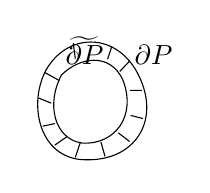
\begin{tikzpicture}[scale=.65]
\draw (0,0) .. controls (-.8,.1) and (-1,1.1) .. (-.65,1.75) .. controls (-.25,2.45) and (.65,2.5) .. (1.1,1.75) .. controls (1.65,.8) and (1.1,-.1) .. (0,0);
\draw (.05,.32) .. controls (-.5,.4) and (-.65,1.1) .. (-.35,1.65) .. controls (0,2) and (.6,2.1) .. (.85,1.55) .. controls (1.12,.85) and (.7,.28) .. (.05,.32);
\draw (-.68,1.7)--(-.39,1.54) (-.8,1.2)--(-.55,1.1) (-.72,.65)--(-.48,.7) (-.48,.28)--(-.25,.44) (-.08,.04)--(.02,.34) (.5,.06)--(.42,.34) (.98,.35)--(.76,.52) (1.24,.8)--(1,.86) (1.22,1.35)--(.99,1.35) (.98,1.92)--(.79,1.72) (.63,2.2)--(.55,1.96) (-.12,2.27)--(-.08,1.97);
\node at (.1,2.12) {$\widetilde{\partial P}$};\node at (1.45,2.05) {$\partial P$};
\end{tikzpicture}}
On a alors \deleted{\unsure{l'isom.} \unsure{à} \unsure{prendre} \unsure{entre}}
\diagram{\begin{tikzcd}[column sep=small]
\deleted{\unsure{\widetilde{\partial P}}}\arrow[r,"{\deleted{\longrightarrow}}" description,draw=none]&\deleted{\unsure{\widetilde{\partial P}}}&\deleted{\partial P'}\arrow[l,"{\deleted{\longleftarrow}}" description,draw=none]&\deleted{P'}\arrow[r,"{\deleted{\longrightarrow}}" description,draw=none]&\deleted{P}
\end{tikzcd}}
\deleted{équivalences d'homotopie}
\mspage{2}
